\documentclass{article}
%\VignetteIndexEntry{Introduction to lexicalStat}
\usepackage{lmodern}
\usepackage{makeidx}
\usepackage{hyperref}
\usepackage[T1]{fontenc}
\usepackage[latin1]{inputenc}
\usepackage{dcolumn}
%\usepackage[francais]{babel}

\makeindex 

\title{Word association measure}

\author{Bernard Desgraupes and Sylvain Loiseau\\
<bernard.desgraupes@u-paris10.fr>, <sylvain.loiseau@univ-paris13.fr>}

\date{\today}

\usepackage{Sweave}
\begin{document}

\maketitle

\begin{abstract}

\end{abstract}

\vspace{5mm}
\hrule
\tableofcontents
\vspace{5mm}
\hrule

\newpage

% ----------------------------------------------------------------
% ----------------------------------------------------------------
%\section{Introduction}
% ----------------------------------------------------------------
% ----------------------------------------------------------------
\label{sec:Intro}

\begin{Schunk}
\begin{Sinput}
> library(wam);
\end{Sinput}
\end{Schunk}

% ----------------------------------------------------------------
% ----------------------------------------------------------------
\section{Indicator of word association}
% ----------------------------------------------------------------
% ----------------------------------------------------------------
\label{sec:indicators}

Each association measure return a numeric vector indicating, for each
corresponding index in the arguments, the association strengh between the word
under scrutiny and the subcorpus.

These association measures, unless otherwise stated in the help page of the
function, are positive when the word is over-represented ("attracted"), and
negative when the word is under-represented.

In absolute value, the more the word is over-representend or under-represented,
the more the association measure givien is hight.

% ................................................................
\subsection{Arguments of the functions}
% ................................................................

All functions have the following signature: ($N$, $n$, $K$, $k$), where:

\begin{enumerate}
	\item $N$ is the total size of the corpora
	\item $n$ is the size of the subcorpora
	\item $K$ is the total frequency of the form under scrutiny in the corpora
	\item $k$ is the sub-frequency of the form under scrutinty in the subcorpora
\end{enumerate}

This can be easily turn into the "contingency table" representation used in some
presentation (according to Stefan Evert UCS documentation) :

\begin{tabular}{llll}
                  word & $� word$ &  T  \\\hline
 subcorpus      & O11  & O12      & R1  \\
                & E11  & E12      &     \\\hline
 $� subcorpus$  & O21  & O22      & R2  \\
                & E21  & E22      &     \\\hline
Totals          & C1   & C2       & N   \\\hline
\end{tabular}

where :

\begin{itemize}
\item         N   = total words in corpus (or subcorpus or restriction, but they are not implemented yet)
\item         C1  = frequency of the collocate in the whole corpus
\item         C2  = frequency of words that aren't the collocate in the corpus
\item         R1  = total words in window
\item         R2  = total words outside of window
\item         O11 = how many of collocate there are in the window 
\item         O12 = how many words other than the collocate there are in the window (calculated from row total)
\item         O21 = how many of collocate there are outside the window
\item         O22 = how many words other than the collocate there are outside the window
\item         E11 = expected values (proportion of collocate that would belong in window if collocate were spread evenly)
\item         E12 =     "    "      (proportion of collocate that would belong outside window if collocate were spread evenly)
\item         E21 =     "    "      (proportion of other words that would belong in window if collocate were spread evenly)
\item         E22 =     "    "      (proportion of other words that would belong outside window if collocate were spread evenly)
\end{itemize}

Conversion from $N$, $n$, $K$, $k$ notation :

\begin{tabular}{llll}
                        & word & $� word$    & $T$   \\
         subcorpus      & $k$    & $n-k$         & $n$   \\
         $� subcorpus$  & $K-k$  & $N-K-(n-k)$   & $N-n$ \\
         Totals         & $K$    & $N-K$         & $N$   \\
\end{tabular}

	
Conversion to $N$, $n$, $K$, $k$ notation :

\itemize{
  \item $N = N$
  \item $n = O11 + O12$
  \item $K = O11 + O21$
  \item $k = O11$
}

We will use the arguments from the data set \emph{robespierre}:

\begin{Schunk}
\begin{Sinput}
> data(robespierre)
> robespierre <- robespierre[1:5,]
> robespierre
\end{Sinput}
\begin{Soutput}
      N    n    K   k      types parts
1 61449 8395 3173 464         de    D1
2 61449 2558  296  45     peuple    D2
3 61449 3920  207  35 republique    D3
4 61449 6903  165  30     ennemi    D4
5 61449 7896  153   6     patrie    D5
\end{Soutput}
\begin{Sinput}
> attach(robespierre)
\end{Sinput}
\end{Schunk}

% ................................................................
\subsection{Recycling arguments}
% ................................................................

Arguments are recycled.

% ................................................................
\subsection{Log-likelihood}
% ................................................................

A given value of attraction between a form and a subcorpus:

\begin{Schunk}
\begin{Sinput}
> wam.loglikelihood(N, n, K, k);
\end{Sinput}
\begin{Soutput}
[1] 5.425296e-02 4.494012e-14 8.616378e-08 4.298495e-03 9.999284e-01
\end{Soutput}
\end{Schunk}

Graph of the function:

\begin{Schunk}
\begin{Sinput}
> plot(wam.loglikelihood(N[1], n[1], K[1], 0:k[1]),
+      type="l", xlab="k", ylab="Log likelihood",
+ 	  main="Graph of the Log likelihood function",
+ 	  sub="(N=61449, n=7896, K=296)")
\end{Sinput}
\end{Schunk}
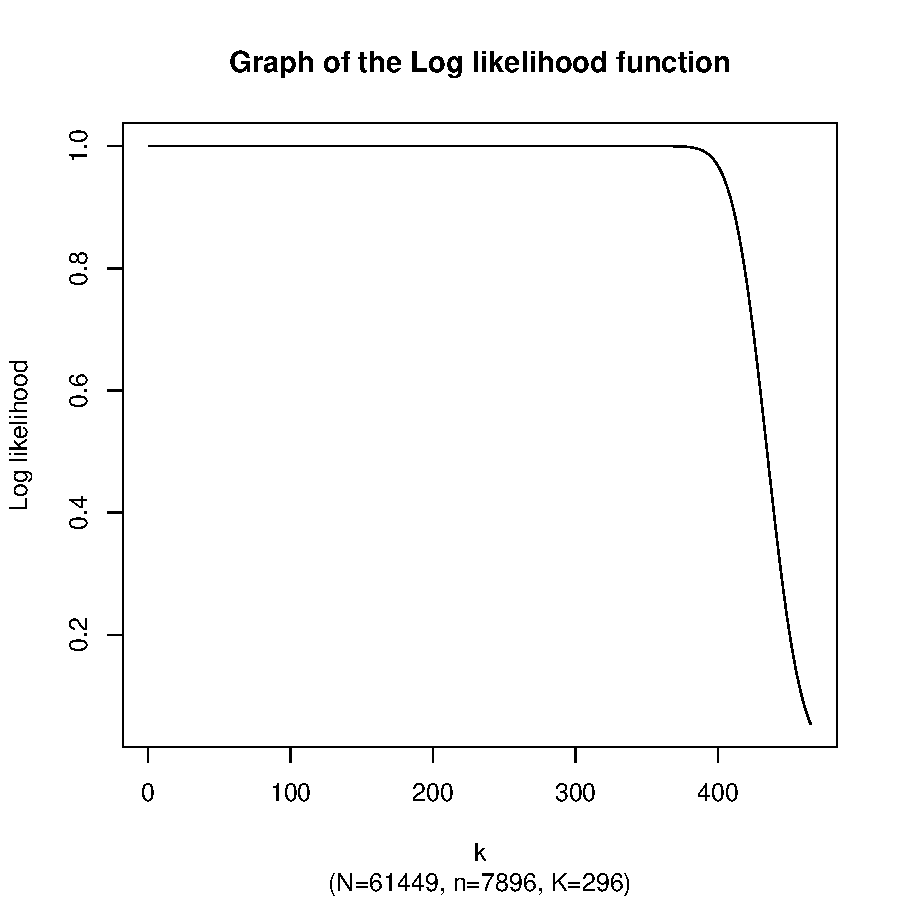
\includegraphics{wam-wam_loglikelihood3}

% ................................................................
\subsection{Specificities}
% ................................................................

This is an implementation of the indicator that has been proposed by Lafon in
"Sur la variabilit� de la fr�quence des formes dans un corpus",
\emph{Mots}, 1, 1980, 127--165
(\url{http://www.persee.fr/web/revues/home/prescript/article/mots_0243-6450_1980_num_1_1_1008}).

A given value of attraction between a form and a subcorpus:

\begin{Schunk}
\begin{Sinput}
> wam.specificities(N, n, K, k);
\end{Sinput}
\begin{Soutput}
[1]  2.184893 29.638212 15.280475  4.544573 -8.037906
\end{Soutput}
\end{Schunk}

Graph of the function:

\begin{Schunk}
\begin{Sinput}
> plot(wam.specificities(N[1], n[1], K[1], 0:k[1], method="base"), type="l", xlab="k", ylab="specificities", main="Graph of the specificities function", sub="(N=61449, n=7896, K=296)")
\end{Sinput}
\end{Schunk}
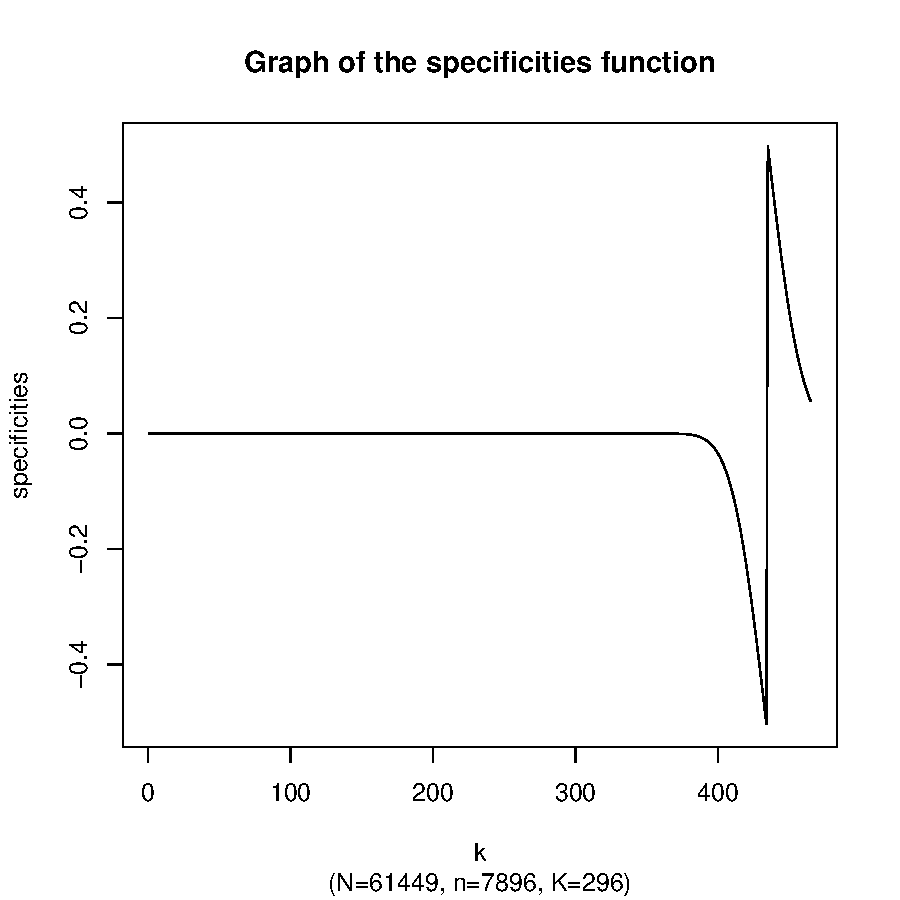
\includegraphics{wam-wam_specificities3}

These exemple is the lexical frequency of the form \emph{peuple} (French for people) in three public discourses
by Robespierre in a corpus of 10 discourses containing $N = 61449$ occurrences in total (Lafon 1980) :

\begin{tabular}{l|rrrr}
Discours & N & n & K & k\\\hline
4 & 61449 & 6903 & 296 & 14  \\
5 & 61449 & 7896 & 296 & 53  \\
8 & 61449 & 2063 & 296 & 16  \\\hline
\end{tabular}

For each line we can compute the expected frequency of the form ($K \times n / N$) and
mark $+$ if the form is more frequent than expected or $-$ otherwise.

\begin{tabular}{l|rrrrrr}\hline
Discours & N & n & K & k & expected & $k > expected$\\\hline
4 & 61449 & 6903 & 296 & 14 & 32.80 & $-$\\ 
5 & 61449 & 7896 & 296 & 53 & 37.52 & $+$\\
8 & 61449 & 2063 & 296 & 16 & 9.80 & $+$\\\hline
\end{tabular}

The form \emph{peuple} is less frequent in the fourth discourse than expected.
On the contrary, \emph{peuple} is more frequent than expected in the fifth and
eigth discourses.

If the observed frequency is less than the expected frequency, we compute the sum of the
probability for a frequency lesser or equal to the observed frequency ($Prob(X \leq k)$).
If the observed frequency is greater than the expected frequency, we compute the sum of the
probability for a frequency greater to the observed frequency ($Prob(X > k)$) (Lafon 1980 : 152).

In both cases, the more unexpected is the frequency, the smaller is the indicator.

\begin{tabular}{l|rrrrrrr}\hline
Discours & N & n & K & k & expected & $k > expected$ & cumulative extreme probability\\\hline
4 & 61449 & 6903 & 296 & 14 & 32.80 & $-$ & 0.0000669371\\
5 & 61449 & 7896 & 296 & 53 & 37.52 & $+$ & 0.0077234888\\
8 & 61449 & 2063 & 296 & 16 & 9.80 & $+$ & 0.0433282491\\\hline
\end{tabular}

According to this indicator, the second case is more "surprising" than the third or, in other
terms, \emph{peuple} is more attracted by, or specific to the second discourse than to the third.

According to relative frequency, one could conclude the other way around:
$ 53 / 7896 = 0.0067 < 16 / 2063 = 0.0078$
(cf. Lafon 1980 : 152).

For the fifth discourse above ($N=61449$, $n=7896$), the possible frequencies of
\emph{peuple} range from $0$ to $296$ (if all occurrences of \emph{peuple}
where in this discours). Here is the corresponding values for the specificities
indicator:

% ................................................................
\subsubsection{Log of specificities}
% ................................................................

The log of the probability; with "-" sign if specificity is negative and "+" if
it is positive.

\begin{Schunk}
\begin{Sinput}
> plot(wam.specificities(N[1], n[1], K[1], 0:k[1], method="log"), type="l", xlab="k", ylab="specificities", main="Specificities indicateur (log)", sub="N=61449, n=7896, K=296")
\end{Sinput}
\end{Schunk}
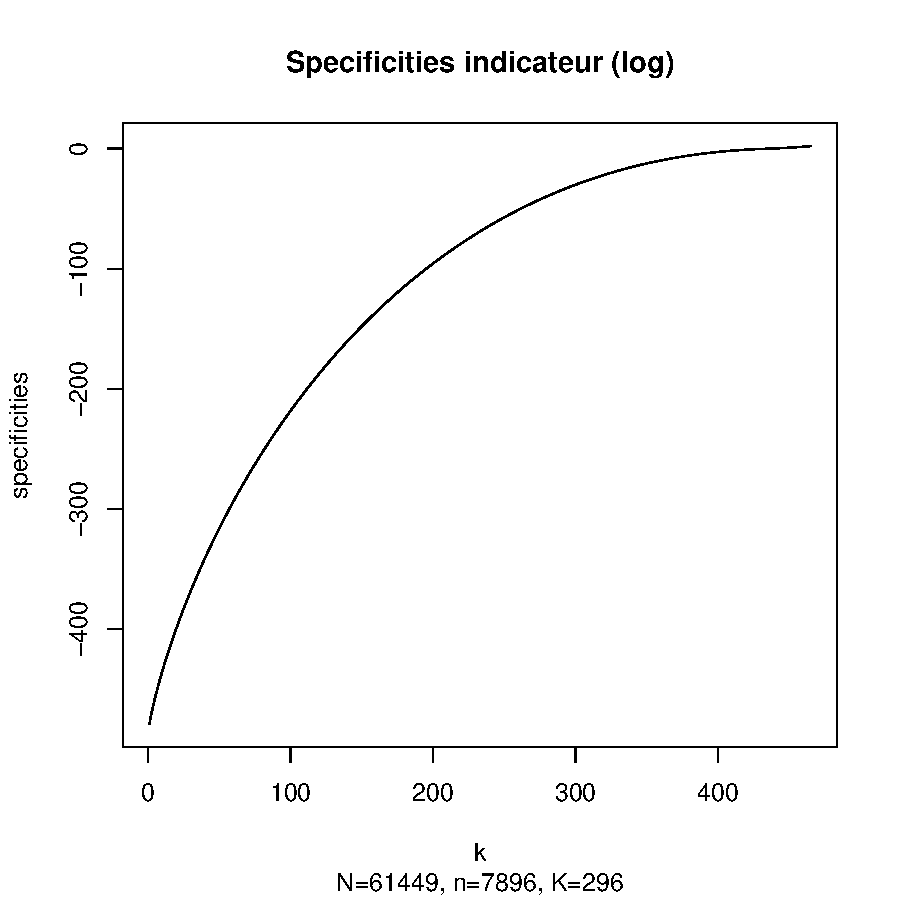
\includegraphics{wam-wam_specificities_log}

% % ----------------------------------------------------------------
% % ----------------------------------------------------------------
% \section{Comparison of indicators}
% % ----------------------------------------------------------------
% % ----------------------------------------------------------------
% \label{sec:comparison-indicators}
%
% TODO
%
% % <<wam_comparison_indicators, echo=FALSE, fig=TRUE>>=
% % par(mfrow=c(1,2))
% % plot(wam.loglikelihood(61449, 7896, 296, 0:296), type="l", xlab="k", ylab="specificities", main="Log likelihood", sub="N=61449, n=7896, K=296")
% % plot(wam.specificities(61449, 7896, 296, 0:296, method="log"), type="l", xlab="k", ylab="specificities", main="Specificities indicateur (log)", sub="N=61449, n=7896, K=296")
% % @

% % ----------------------------------------------------------------
% % ----------------------------------------------------------------
% \section{Distribution of the specificities of a form across sub-corpus}
% % ----------------------------------------------------------------
% % ----------------------------------------------------------------
% \label{sec:distribution-subcorpus}
%
% TODO
%
% <<wam_distribution, echo=FALSE, fig=FALSE>>=
% #library(rcqp);
% #c <- corpus("DICKENS");
% #x <- cqp_ftable(c, "book", "lemma");
% #z <- cast(x, lemma~book, fun.aggregate=sum, value="freq")
% #F <- rowSums(z);
% #
% ##N <- sum(x$freq);
% ##f <- x[x[,1] == "1", "freq"];
% ##l <- x[x[,1] == "1", "lemma"];
% ##n <- sum(f);
% ##F <- rowSums(x);
% #s <- wam.specificities(sum(F), sum(z[1]), F, x[1])
% #hist(s, breaks=100);
% @

% ----------------------------------------------------------------
% ----------------------------------------------------------------
\section{High level interface}
% ----------------------------------------------------------------
% ----------------------------------------------------------------
\label{sec:indicators}

The function \emph{wam} provide a more high level interface to the actual functions.

This function allows for computing several indicator at the same time.

It takes also as argument the subcorpus name and lexical types.

\begin{Schunk}
\begin{Sinput}
> attach(robespierre)
> wam.res <- wam(N, n, K, k, measure=c("loglikelihood", "specificities"), parts, types)
\end{Sinput}
\end{Schunk}

function allows for retrieving the basic information:

\begin{Schunk}
\begin{Sinput}
> attach(robespierre)
> wam.res <- wam(N, n, K, k, measure=c("loglikelihood", "specificities"), parts, types)
\end{Sinput}
\end{Schunk}

A print implementation allows for an easy to use reading of the results:

\begin{Schunk}
\begin{Sinput}
> attach(robespierre)
> wam.res <- wam(N, n, K, k, measure=c("loglikelihood", "specificities"), parts, types)
> wam.res
\end{Sinput}
\begin{Soutput}
Printing association measure for 5 part(s); from: 1 to: 100 
Corpus size: 61449 
Sorted by: loglikelihood 
-------------------------------------------------------------------------------
word                 | sub freq | tot freq |   loglikelihood |   specificities 
-------------------------------------------------------------------------------
...............................................................................
Part name: de 
Part size: 8395 tokens. 
Positive specificities printed: 1 
Negative specificities printed: 0 
D1                   |      464 |     3173 |            0.05 |            2.18 
...............................................................................
Part name: ennemi 
Part size: 6903 tokens. 
Positive specificities printed: 1 
Negative specificities printed: 0 
D4                   |       30 |      165 |            0.00 |            4.54 
...............................................................................
Part name: patrie 
Part size: 7896 tokens. 
Positive specificities printed: 1 
Negative specificities printed: 0 
D5                   |        6 |      153 |            1.00 |           -8.04 
...............................................................................
Part name: peuple 
Part size: 2558 tokens. 
Positive specificities printed: 1 
Negative specificities printed: 0 
D2                   |       45 |      296 |            0.00 |           29.64 
...............................................................................
Part name: republique 
Part size: 3920 tokens. 
Positive specificities printed: 1 
Negative specificities printed: 0 
D3                   |       35 |      207 |            0.00 |           15.28 
\end{Soutput}
\end{Schunk}

% ----------------------------------------------------------------
% ----------------------------------------------------------------
\section{Bibliographie}
% ----------------------------------------------------------------
% ----------------------------------------------------------------

Dunning, T. 1993. "Accurate methods for the statistics of surprise and coincidence." In: Computational Linguistics. 19(1). Pp 61--74.

\url{http://acl.ldc.upenn.edu/J/J93/J93-1003.pdf}

Hofland, K. and Johanssen, S. 1989. Frequency analysis of English vocabulary and grammar, based on the LOB corpus. Oxford: Clarendon.

Kilgarriff, A. 1996. "Which words are particularly characteristic of a text? A survey of statistical approaches." In: Proceedings, ALLC-ACH '96. Bergen, Norway.

\url{http://www.cse.iitb.ac.in/~shwetaghonge/prec_recall.pdf}

Chaudhari, D. L., Damani, O. P. \& Laxman, S. 2011. "Lexical co-occurrence, statistical significance, and word association". In: Conference on Empirical Methods in Natural Language Processing (Edinburgh, Scotland, UK, July 27-31).
pp. 1058-68

\url{http://www.aclweb.org/anthology-new/D/D11/D11-1098.pdf}

\printindex

\end{document}

